% Graphic for TeX using PGF
% Title: C:\Users\Louis\Desktop\Projet Fiches\Figures\bilans\blocs.dia
% Creator: Dia v0.97.2
% CreationDate: Fri Aug 07 19:05:29 2015
% For: Louis
% \usepackage{tikz}
% The following commands are not supported in PSTricks at present
% We define them conditionally, so when they are implemented,
% this pgf file will use them.
\ifx\du\undefined
  \newlength{\du}
\fi
\setlength{\du}{15\unitlength}
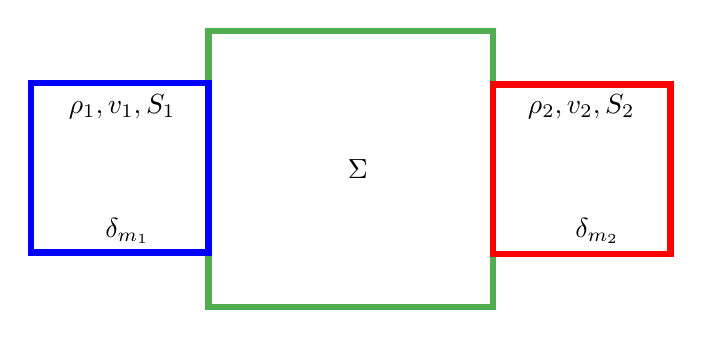
\begin{tikzpicture}[scale=0.4]
\pgftransformxscale{1.000000}
\pgftransformyscale{-1.000000}
\definecolor{dialinecolor}{rgb}{0.000000, 0.000000, 0.000000}
\pgfsetstrokecolor{dialinecolor}
\definecolor{dialinecolor}{rgb}{1.000000, 1.000000, 1.000000}
\pgfsetfillcolor{dialinecolor}
\pgfsetlinewidth{0.150000\du}
\pgfsetdash{}{0pt}
\pgfsetdash{}{0pt}
\pgfsetmiterjoin
\definecolor{dialinecolor}{rgb}{1.000000, 1.000000, 1.000000}
\pgfsetfillcolor{dialinecolor}
\fill (27.500000\du,12.950000\du)--(27.500000\du,29.600000\du)--(44.650000\du,29.600000\du)--(44.650000\du,12.950000\du)--cycle;
\definecolor{dialinecolor}{rgb}{0.321569, 0.674510, 0.321569}
\pgfsetstrokecolor{dialinecolor}
\draw (27.500000\du,12.950000\du)--(27.500000\du,29.600000\du)--(44.650000\du,29.600000\du)--(44.650000\du,12.950000\du)--cycle;
\pgfsetlinewidth{0.150000\du}
\pgfsetdash{}{0pt}
\pgfsetdash{}{0pt}
\pgfsetmiterjoin
\definecolor{dialinecolor}{rgb}{1.000000, 1.000000, 1.000000}
\pgfsetfillcolor{dialinecolor}
\fill (16.800000\du,16.100000\du)--(16.800000\du,26.300000\du)--(27.500000\du,26.300000\du)--(27.500000\du,16.100000\du)--cycle;
\definecolor{dialinecolor}{rgb}{0.000000, 0.000000, 1.000000}
\pgfsetstrokecolor{dialinecolor}
\draw (16.800000\du,16.100000\du)--(16.800000\du,26.300000\du)--(27.500000\du,26.300000\du)--(27.500000\du,16.100000\du)--cycle;
\pgfsetlinewidth{0.150000\du}
\pgfsetdash{}{0pt}
\pgfsetdash{}{0pt}
\pgfsetmiterjoin
\definecolor{dialinecolor}{rgb}{1.000000, 1.000000, 1.000000}
\pgfsetfillcolor{dialinecolor}
\fill (44.630000\du,16.185000\du)--(44.630000\du,26.385000\du)--(55.330000\du,26.385000\du)--(55.330000\du,16.185000\du)--cycle;
\definecolor{dialinecolor}{rgb}{1.000000, 0.000000, 0.000000}
\pgfsetstrokecolor{dialinecolor}
\draw (44.630000\du,16.185000\du)--(44.630000\du,26.385000\du)--(55.330000\du,26.385000\du)--(55.330000\du,16.185000\du)--cycle;
% setfont left to latex
\definecolor{dialinecolor}{rgb}{0.000000, 0.000000, 0.000000}
\pgfsetstrokecolor{dialinecolor}
\node[anchor=west] at (35.150000\du,21.250000\du){$\Sigma$};
% setfont left to latex
\definecolor{dialinecolor}{rgb}{0.000000, 0.000000, 0.000000}
\pgfsetstrokecolor{dialinecolor}
\node[anchor=west] at (18.350000\du,17.50000\du){$\rho_{1},v_{1},S_{1}$};
% setfont left to latex
\definecolor{dialinecolor}{rgb}{0.000000, 0.000000, 0.000000}
\pgfsetstrokecolor{dialinecolor}
\node[anchor=west] at (46.000000\du,17.50000\du){$\rho_{2},v_{2},S_{2}$};
% setfont left to latex
\definecolor{dialinecolor}{rgb}{0.000000, 0.000000, 0.000000}
\pgfsetstrokecolor{dialinecolor}
\node[anchor=west] at (20.550000\du,25.000000\du){$\delta_{m_{1}}$};
% setfont left to latex
\definecolor{dialinecolor}{rgb}{0.000000, 0.000000, 0.000000}
\pgfsetstrokecolor{dialinecolor}
\node[anchor=west] at (48.850000\du,25.000000\du){$\delta_{m_{2}}$};
\end{tikzpicture}
